%!TEX root = ../../../tugas-akhir.tex
\section{Implementasi Algoritma Paralel pada Library big integer}
\subsection{Lingkungan Implementasi} \label{sec:impl_env}
Sesuai dengan pertimbangan pada subbab \ref{sec:parallel_env}, implementasi algoritma paralel akan dilakukan dengan menggunakan pthread. Implementasi akan dilakukan menggunakan \textit{compiler} GCC versi 5.4.0 dan dijalankan pada sistem operasi Ubuntu 18.04 64-bit. Penggunaan TLS akan diuji pada penggunaan HTTPS pada web server yang diinstall pada sistem operasi. Web server yang digunakan adalah Apache2 dengan menggunakan modul tambahan mod\_ssl. Arsitektur sistem yang digunakan dapat dilihat pada Gambar \ref{fig:openssl_arch}

\begin{figure}[h]
  \centering
  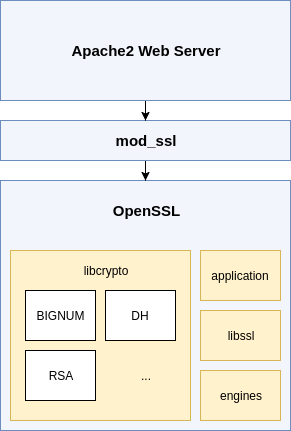
\includegraphics[width=0.4\textwidth]{resources/ch-4/implementation_arch.png}
  \caption{Arsitektur OpenSSL}
  \label{fig:openssl_arch}
\end{figure}

% Cek lagi jumlahnya
Secara default, jumlah maksimal thread maksimum yang akan digunakan oleh OpenSSL untuk menjalankan komputasi big integer secara paralel akan bergantung pada jumlah core yang terdapat pada lingkungan instalasi. Dalam aplikasi yang membutuhkan komputasi yang tinggi setiap thread akan berjalan secara terus menerus. Dengan demikian jumlah thread maksimum akan sama dengan jumlah aplikasi. Namun, aplikasi juga memiliki pilihan konfigurasi untuk menentukan jumlah thread maksimum yang dapat digunakan.
% \todo{cite disini}

\subsection{Batasan Implementasi}
Implementasi dilakukan pada sistem operasi Ubuntu 64 bit. Karena itu, implementasi library big number hanya berfokus pada openssl dengan yang memiliki konfigurasi makro sebagai berikut:
\begin{enumerate}[label=\roman*.]
  \item BN\_ULONG = unsigned long long
  \item OPENSSL\_SMALL\_FOOTPRINT = false
  \item BN\_MUL\_COMBA = true
  \item BN\_RECURSION = true

\end{enumerate}

Konfigurasi makro tersebut digunakan dalam pemilihan dan manajemen struktur data yang digunakan serta pemilihan algoritma pada bagian tertentu. Sebagai contoh, algoritma yang digunakan dalam perkalian adalah algoritma karatsuba dan algoritma comba pada basis rekursif.

\subsection{Struktur Data Big Integer} \label{sec:bignum_struct}
Pada OpenSSL, sebuah big integer direpresentasikan dalam struktur data BIGNUM. BIGNUM terdiri dari sebuah array dengan ukuran dinamis dan beberapa integer yang menyimpan informasi tambahan. Dengan demikian secara teori BIGNUM tidak memiliki nilai maksimum. Untuk keperluan paralelisasi, BIGNUM dapat digunakan tanpa mengubah strukturnya sedikitpun. BIGNUM sendiri merupakan sebuah \textit{struct} yang memiliki deklarasi sebagai berikut.

\begin{lstlisting}[caption=Struktur Data bignum]
struct bignum_st {
       BN_ULONG *d;
       int top;
       int dmax;
       int neg;
       int flags;
};
\end{lstlisting}

|BN_ULONG| sendiri adalah sebuah makro yang menggantikan |unsigned long| pada komputer 32 bit atau |unsigned long long| pada komputer 64 bit.

|d| adalah pointer untuk array of integer.

|top| merupakan index |d| yang terakhir digunakan plus satu.

|dmax| adalah panjang maksimum array yang telah dibuat. |neg| bernilai satu jika BIGNUM bernilai negatif.

\todo[inline]{jelasin BN\_CTX}

\subsection{Struktur File \textit{Source Code}}

\missingfigure{Struktur file}

Struktur \textit{source code} dapat dilihat pada Gambar XXX. Direktori utama berisi pembagian dari fungsi aplikasi yang ada dalam OpenSSL. Beberapa fungsi tersebut adalah direktori |doc| yang berisi dokumentasi OpenSSL, |crypto| yang berisi library kriptografi, |ssl| yang berisi dari library komunikasi ssl, serta |test| yang berisi unit test yang dimiliki OpenSSL.

Direktori |crypto| berisi modul-modul yang membentuk libcrypto, dengan setiap modul terbentuk dalam sebuah direktori yang berbeda. Modul |bn| merupakan modul yang mengatasi perhitungan operasi aritmatika big integer. Selain itu, modul |dh| dan |rsa| merupakan modul yang menangani komputasi Diffie-Hellman dan RSA pada OpenSSL.

Modul |bn| memiliki beberapa submodul masing-masing merupakan file yang berbeda. Setiap submodul sendiri mengatasi fungsi yang terkait dengan submodul tersebut, ataupun operasi yang komputasinya mirip dengan submodul. Sebagai contoh, submodul |bn_add| merupakan submodul yang mengatasi operasi penjumlahan dan pengurangan pada big integer. Selain itu, submodul |bn_mul| merupakan submodul yang mengatasi operasi perkalian serta pemilihan algoritma perkalian yang digunakan dalam OpenSSL.

\subsection{Modul Operasi Aritmatika}
\subsubsection{Submodul Penjumlahan dan Pengurangan}
Modul penjumlahan dan pengurangan terdapat pada file BN\_add.c. Fungsi BN\_add() pada modul ini melakukan pengolahan data pada a dan b seperti mengecek negatif dan mengecek panjang masing-masing array. Hasil pengecekan tersebut akan digunakan untuk melakukan operasi lebih lanjut. Jika a dan b memiliki tanda yang berbeda, akan dipanggil fungsi BN\_usub() selain itu akan dipanggil fungsi BN\_uadd(). BN\_uadd() dan BN\_usub() melakukan pengolahan data pada a dan b sehingga terdapat representasi array yang dapat diolah oleh BN\_add\_words() dan BN\_sub\_words(). Daftar fungsi yang terdapat pada submodul penjumlahan dan pengurangan dapat dilihat pada Tabel \ref{tab:bn_add_func}.

BN\_add\_words merupakan fungsi yang menerima masukan dua array dengan ukuran yang sama dan menjumlahkannya secara sekuensial. Penerapan algoritma \ref{alg:add} pada OpenSSL terdapat pada fungsi ini.

\begin{table}[!h]
  \caption{Fungsi dalam submodul bn\_add}
  \label{tab:bn_add_func}
  \begin{tabular}{R{2.5cm}L{10.5cm}}
\toprule
\textbf{Header Fungsi} & |int BN_add(BIGNUM *r, const BIGNUM *a, const BIGNUM *b)|    \\ \midrule
\textit{Deskripsi}    & Menjumlahkan a dan b dan menyimpan hasilnya pada r $(a+b=r)$ \\
\textit{Prekondisi}    & - \\
\textit{Return Value}  & 1 jika fungsi berhasil dilakukan dan 0 jika tidak
 \\ \bottomrule
\textbf{Header Fungsi} & |int BN_sub(BIGNUM *r, const BIGNUM *a, const BIGNUM *b)|    \\ \midrule
\textit{Deskripsi}    & Mengurangi b dari a dan menyimpan hasilnya pada r $(a-b=r)$ \\
\textit{Prekondisi}    & - \\
\textit{Return Value}  & 1 jika fungsi berhasil dilakukan dan 0 jika tidak
 \\ \bottomrule
\textbf{Header Fungsi} & |int BN_uadd(BIGNUM *r, const BIGNUM *a, const BIGNUM *b)|    \\ \midrule
\textit{Deskripsi}    & Menjumlahkan a dan b dan menyimpan hasilnya pada r $(a+b=r)$ \\
\textit{Prekondisi}    & $a \geq 0$,$ b \geq 0$ \\
\textit{Return Value}  & 1 jika fungsi berhasil dilakukan dan 0 jika tidak
 \\ \bottomrule
\textbf{Header Fungsi} & |int BN_usub(BIGNUM *r, const BIGNUM *a, const BIGNUM *b)|    \\ \midrule
\textit{Deskripsi}    & Mengurangi b dari a dan menyimpan hasilnya pada r $(a-b=r)$ \\
\textit{Prekondisi}    & $a \geq 0$, $b \geq 0$, $a \geq b$ \\
\textit{Return Value}  & 1 jika fungsi berhasil dilakukan dan 0 jika tidak
 \\ \bottomrule
\end{tabular}

\end{table}

\subsubsection{Modul Perkalian}
\begin{table}[h]
  \caption{Fungsi dalam submodul bn\_add}
  \begin{tabular}{R{2.5cm}L{10.5cm}}
\toprule
\textbf{Header Fungsi} & |int BN_mul(BIGNUM *r, const BIGNUM *a, const BIGNUM *b, BN_CTX *ctx)|    \\ \midrule
\textit{Deskripsi}     & Mengalikan $b$ pada $a$ dan menyimpan hasilya dalam $r, (r = a * b)$. \\
\textit{Prekondisi}    & - \\
\textit{Return Value}  & 1 jika fungsi berhasil dilakukan dan 0 jika tidak
 \\ \bottomrule
\textbf{Header Fungsi} & |void bn_mul_normal(BN_ULONG *r, BN_ULONG *a, int na, BN_ULONG *b, int nb)|    \\ \midrule
\textit{Deskripsi}     &  Perkalian $a$ dan $b$ dengan menggunakan algoritma perkalian panjang, dengan $na$ adalah panjang $a$ dan $nb$ adalah panjang $b$.\\
\textit{Prekondisi}    &  -\\
\textit{Return Value}  & 1 jika fungsi berhasil dilakukan dan 0 jika tidak
 \\ \bottomrule
\textbf{Header Fungsi} & |void bn_mul_recursive(BN_ULONG *r, BN_ULONG *a, BN_ULONG *b, int n2 int dna, int dnb, BN_ULONG *t)|    \\ \midrule
\textit{Deskripsi}     &  Perkalian $a$ dan $b$ dengan menggunakan algoritma perkalian karatsuba. $n2$ adalah panjang hasil perkalian, dengan $dna = length(a) - n2$ dan $dnb = length(b) - n2$\\
\textit{Prekondisi}    & $length(r) = 2*n2$. $ length(t) = 2*n2$. $n2 = 2^k, k \in \mathbb{Z}. $\\
\textit{Return Value}  & 1 jika fungsi berhasil dilakukan dan 0 jika tidak
 \\ \bottomrule
\end{tabular}

\end{table}

\subsubsection{Submodul Pembagian}
\begin{table}[h]
  \caption{Fungsi dalam submodul bn\_add}
  \begin{tabular}{R{2.5cm}L{10.5cm}}
\toprule
\textbf{Header Fungsi} & |BN_div(BIGNUM *dv, BIGNUM *rm, const BIGNUM *num, const BIGNUM *divisor, BN_CTX *ctx)|    \\ \midrule
\textit{Deskripsi}     &  Membagi num dengan divisor, hasil pembagian disimpan sebagai dv dan sisa pembagian disimpan sebagai rm. Baik div maupun rm bisa menjadi NULL jika hasil atau sisa pembagian tidak dibutuhkan. \\
\textit{Prekondisi}    &  -\\
\textit{Return Value}  &1 jika fungsi berhasil dilakukan dan 0 jika tidak
 \\ \bottomrule
\textbf{Header Fungsi} & |int bn_left_align(BIGNUM *num)|    \\ \midrule
\textit{Deskripsi}     &  Normalisasi BIGNUM $num$ agar $num > \beta/2$\\
\textit{Prekondisi}    & - \\
\textit{Return Value}  & 1 jika fungsi berhasil dilakukan dan 0 jika tidak
 \\ \bottomrule
\end{tabular}

\end{table}
